The problem of taxonomy classification of product titles is central to an e-commerce organization. 
Large online e-commerce companies usually obtain millions of new listing feeds per month from several hundred merchants subscribed to use proprietary ``publish $\rightarrow$ search $\rightarrow$ buy'' platforms specific to each of these companies. 
The ease of use, control on data quality and organization and functionality of these platforms are the key factors for differentiating the success of the revenue generation model for the companies.

The sale of product listings within an e-commerce platform is critically dependent upon end users being able to search for the correct product using some minimal to advanced search functionality provided by the developers of the platform. 
In this paper we differentiate products from product listings using a simple example. 
Consider a product with a title of ``\textit{Wilson tennis racket Level 3 signed by Federer}''. 
Merchant \textbf{A} can list this product with a title of ``\textit{Wilson tennis racquet Level 3 Roger Federer}''' and with a list price of \$80 while merchant \textbf{B} can list the same product with its original title but with a list price of \$72.
The e-commerce platform keeps track of these two product items as two different listings although they are the same product after some title text disambiguation.
Similar examples occur in thousands for product titles having the same title text but differing in price and/or other fields.
Title text disambiguation in absence of any global identifier for products is also a core-problem in e-commerce platforms that follow an online marketplace model, but we do not address that problem here.
In this paper, we will refer to product listings as listings henceforth. 

Most e-commerce companies keep track of high Gross Merchandise Sales (GMS) products and tune search results to queries conditional on GMS and other meta features such as clickstream as well as  content specific features.
One such critical meta feature is the taxonomy classification of listings.
On a web search platform, categories of search results have already been used to improve web query classification \cite{Ganti10} and such kind of query classifications are also very useful for product search engines.
Further, clues from taxonomies have are very useful in user persona detection and targeted campaigns, recommendations, clustering of  ranked lists of listings and many other applications.

\begin{figure}[ht]
	\centering
	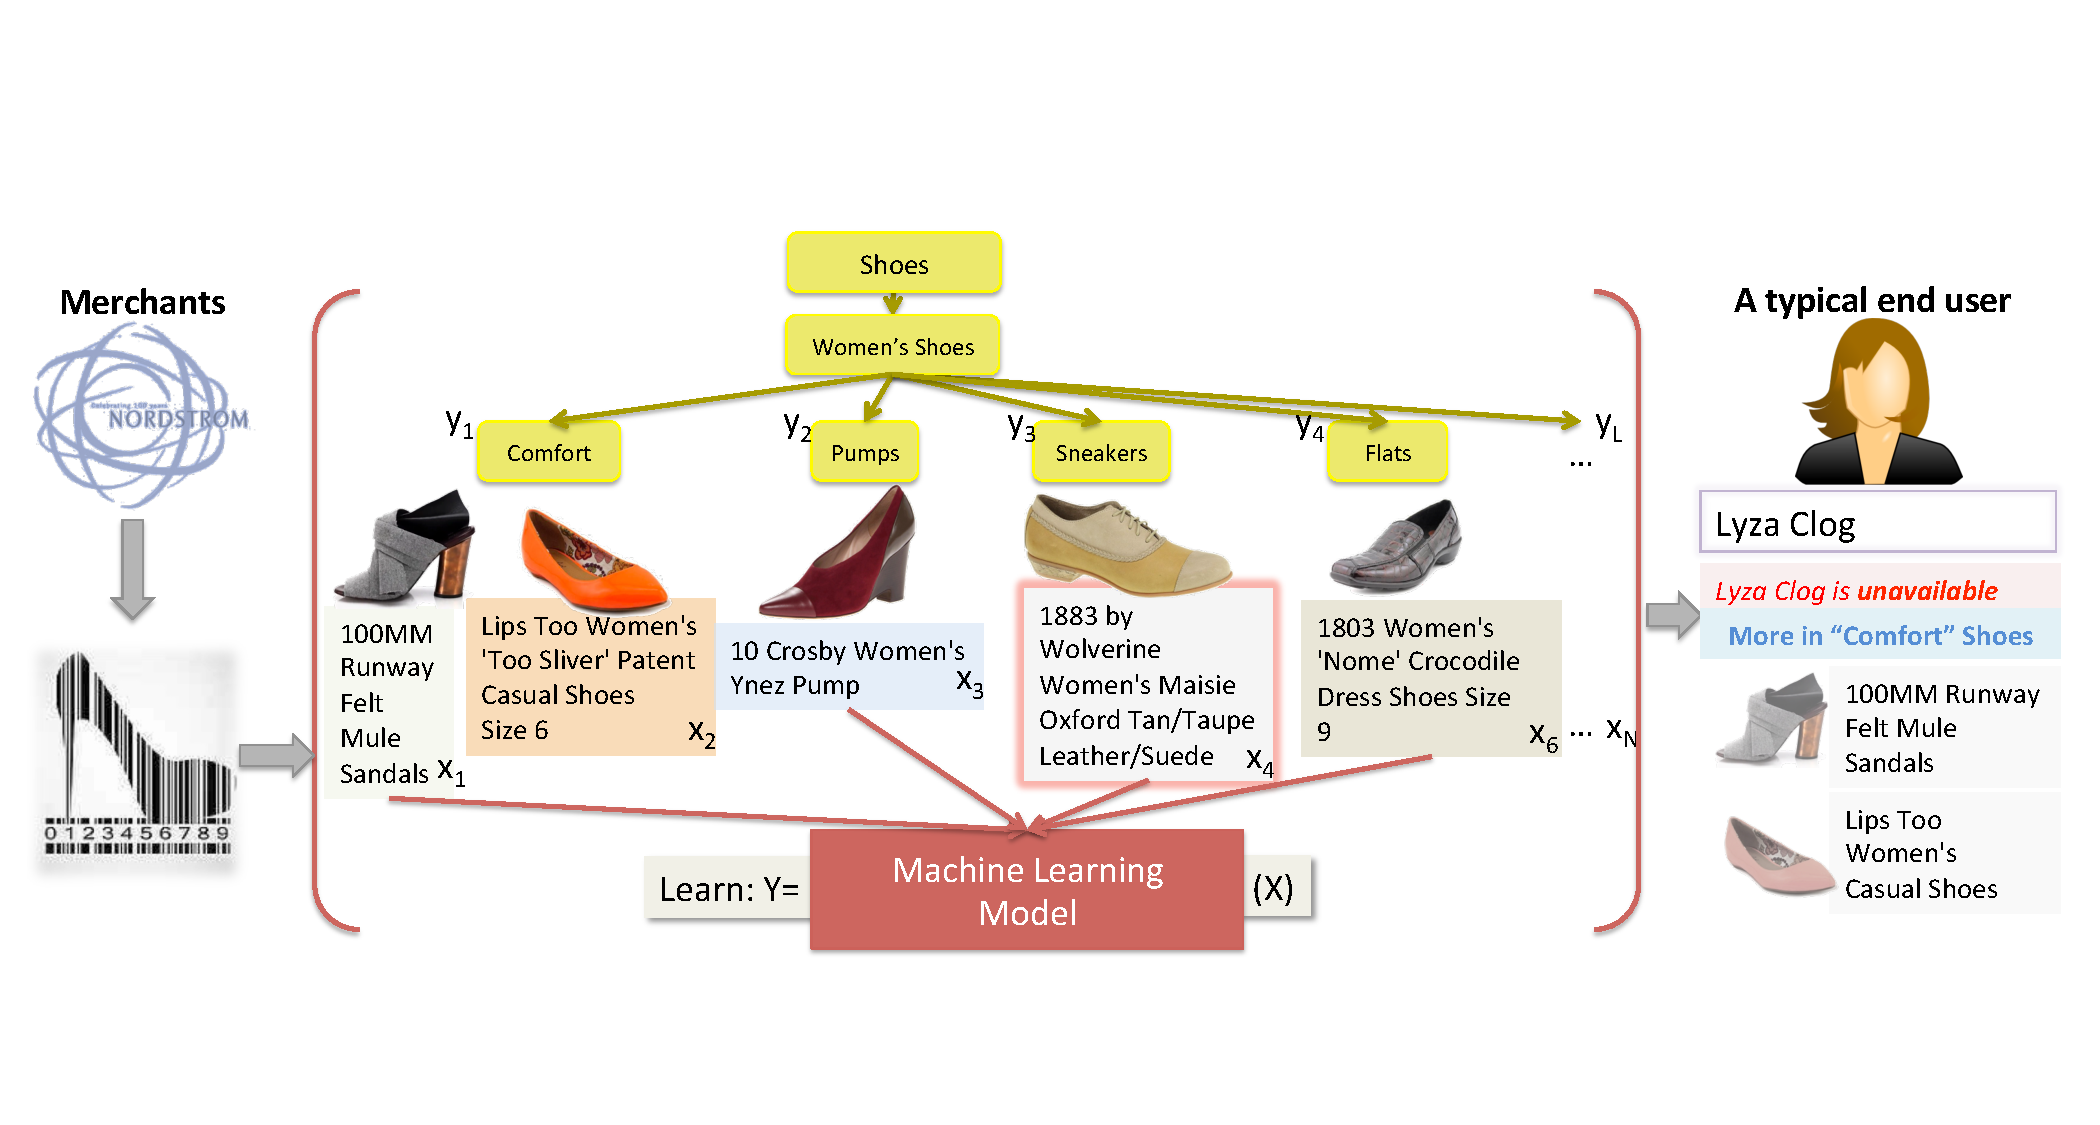
\includegraphics[width=0.9\textwidth]{images/push-pull}
	\vspace{-0.2cm}
	\caption{{\small Merchants push new listings to a data organization and search platform. The listings are then annotated in various ways including a core taxonomy categorization component. The indexed listings together with the annotations influence search and other data organization algorithms. The relevance of the information that end users pull from the indexing platform determines the eventual conversion and revenue generation effectiveness of the e-commerce platform. In this example, taxonomy classification can be very helpful even though the item searched for is not available.}}
	\label{Fig:push-pull}
\end{figure}
\vspace{-0.5cm}

In this paper, we focus on taxonomy classifications of listings in order to solve problems arising in the scenario described in Fig. \ref{Fig:push-pull}.
Generally, merchants interested in publishing their listings to an online e-commerce platform, pushes their feed to an intelligent indexing engine which then are ready to be consumed by the end user in a variety of ways.
Feeds usually come in at 10-20 million listings/day for mid scale e-commerce companies.
Taxonomy categorization of listings is often the first core annotation step for these platforms.

In large e-commerce companies that follow the marketplace models of business to business to customer (B2B2C) commerce, such as Rakuten, creating an maintaining an unified product taxonomy a.k.a product catalog is very difficult. 
This can happen for many reasons including differences in opinions, cross-border trading and more importantly acquisitions of external companies that are profitable and niche.
Each of the acquired companies have their own taxonomies and although they are merged under a common parent company, they operate as independent Business Units (BUs) with their own data feeds and data organization algorithms for some time.
In this paper, we perform experiments on listings data from two such BUs -- BU1 and BU2 -- belonging to Rakuten USA Inc.
which is managed by Rakuten Ichiba, the largest e-commerce company in Japan.

Dataset characteristics vary substantially from BU to BU.
Data from BU1 is substantially corrected using large scale human annotation efforts, contracted to BU1 only, in terms of crafting rules for categorization.
This leads to lower coverage at the expense of high precision and much lower noise, however, such kind of manual efforts are not scalable.
On the other hand, the listing feed which BU2 receives is from external data vendors who sell their feed at substantial subscription rates. 
Moreover, even with their pricing, the taxonomies and categorization they provide are often wrong.
BU2 converts taxonomies from these data vendors to their own manually and hence directly maps listings without any error correction.
We observe such instances of error in Fig. \ref{Fig:push-pull} for the leaf node ``\textbf{Sneakers}'' and the listing ``\textit{1883 by Wolverine Women's Maisie Oxford Tan/Taupe Leather/Suede}'' - the correct leaf node should have been ``\textbf{Oxfords}'' (not shown in Fig. \ref{Fig:push-pull}).

In our scenario, due to the absence of a ground-truth training set from BU2, we rely on this dataset for training our classifiers. 
Automatic categorizations are continuously eliminated manually either in-house (low budget) or through external organizations such as CrowdFlower\footnote{\scriptsize{\url{https://www.crowdflower.com/crowdflower-attacks-data-scientists-biggest-challenge-incomplete-messy-data/}}}.
Needless to mention, the amount of this kind of ``label flip'' error is not nominal and it is hard to correct these without manual scans of millions of listings -- an impossible task which is mitigated to some extent for BU2's dataset using topic model based noise analysis (see Section \ref{Subsect:BU2-noise-analysis}).
Dataset imbalance is also a major problem in product listing datasets for building classification models.
Most loss functions that are not resistant to imbalance generalize very poorly without resorting to any subsampling techniques \cite{Chawla02:SMOTE}. 
We, instead, resort to cross-entropy (logistic) loss functions which are more resistant to imbalance particularly with suitable regularizers (see Section \ref{Sect:results}). 

\begin{wrapfigure}{r}{0.42\textwidth}
	\centering
	\vspace{-0.6cm}
	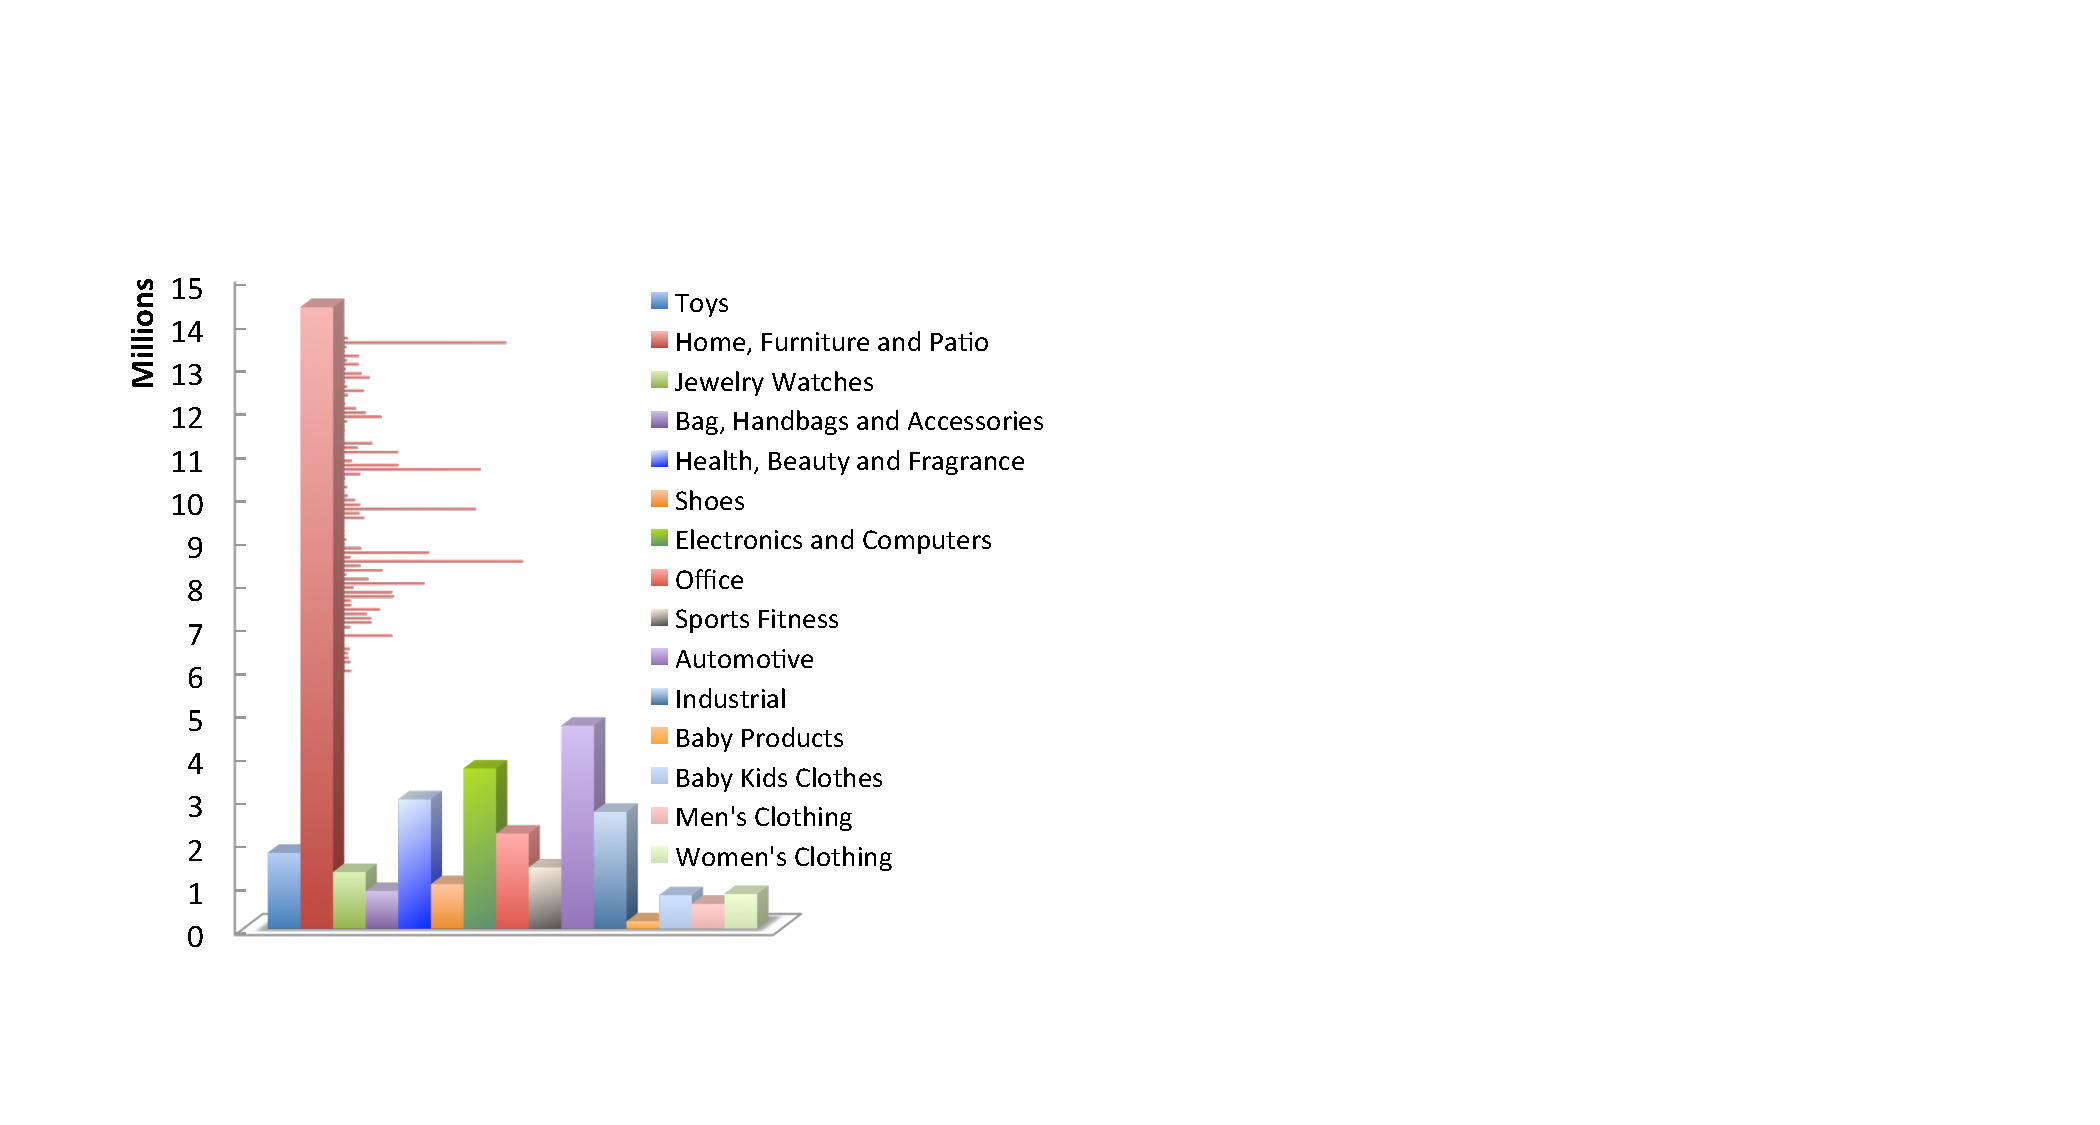
\includegraphics[width=0.42\textwidth]{images/BU2-dataset-Dec2015}
	\vspace{-0.6cm}
	\caption{{\small Dataset from BU2 -- Dec 2015 snapshot. Total number of de-duplicated listings is 40 million.}}
	\vspace{-0.6cm}
	\label{Figure_BU2-datset-earlier}
\end{wrapfigure}
A preview of the imbalance in BU2's dataset can be viewed in Fig. \ref{Figure_BU2-datset-earlier}.  
This dataset has a disproportionate number of listings falling into the ``Home, Patio and Furniture'' category.
However, since BU2 gets its listing feed from external crawls and vendor's taxonomy assignments, it is hard to determine the exact reason behind the imbalance. 
In the experiments shown in Section \ref{Sect:results}, we use BU2's data snapshot from Feb 2016 which consists of 204 million deduplicated listings from 277 merchants and 60 million listings after aggressive cleanup (see Section \ref{Subsect:BU2-noise-analysis}).

In this paper, we solve the taxonomy classification problem as a bi-level problem.
For example, in the case of BU2 dataset, a test listing is first classified into one of the level one classes shown in the legend in Fig. \ref{Figure_BU2-datset-earlier}.
It is then classified by the model corresponding to the level one taxonomy subtrees identified by the level one root nodes such as ``Toys'', ``Home, Furniture and Patio'' etc.
We found this scheme to be more effective in preventing error snowballing effect in the case of a truly level-by-level cascading classification scheme.
\begin{wrapfigure}{l}{0.45\textwidth}
	\centering
	\vspace{-0.6cm}
	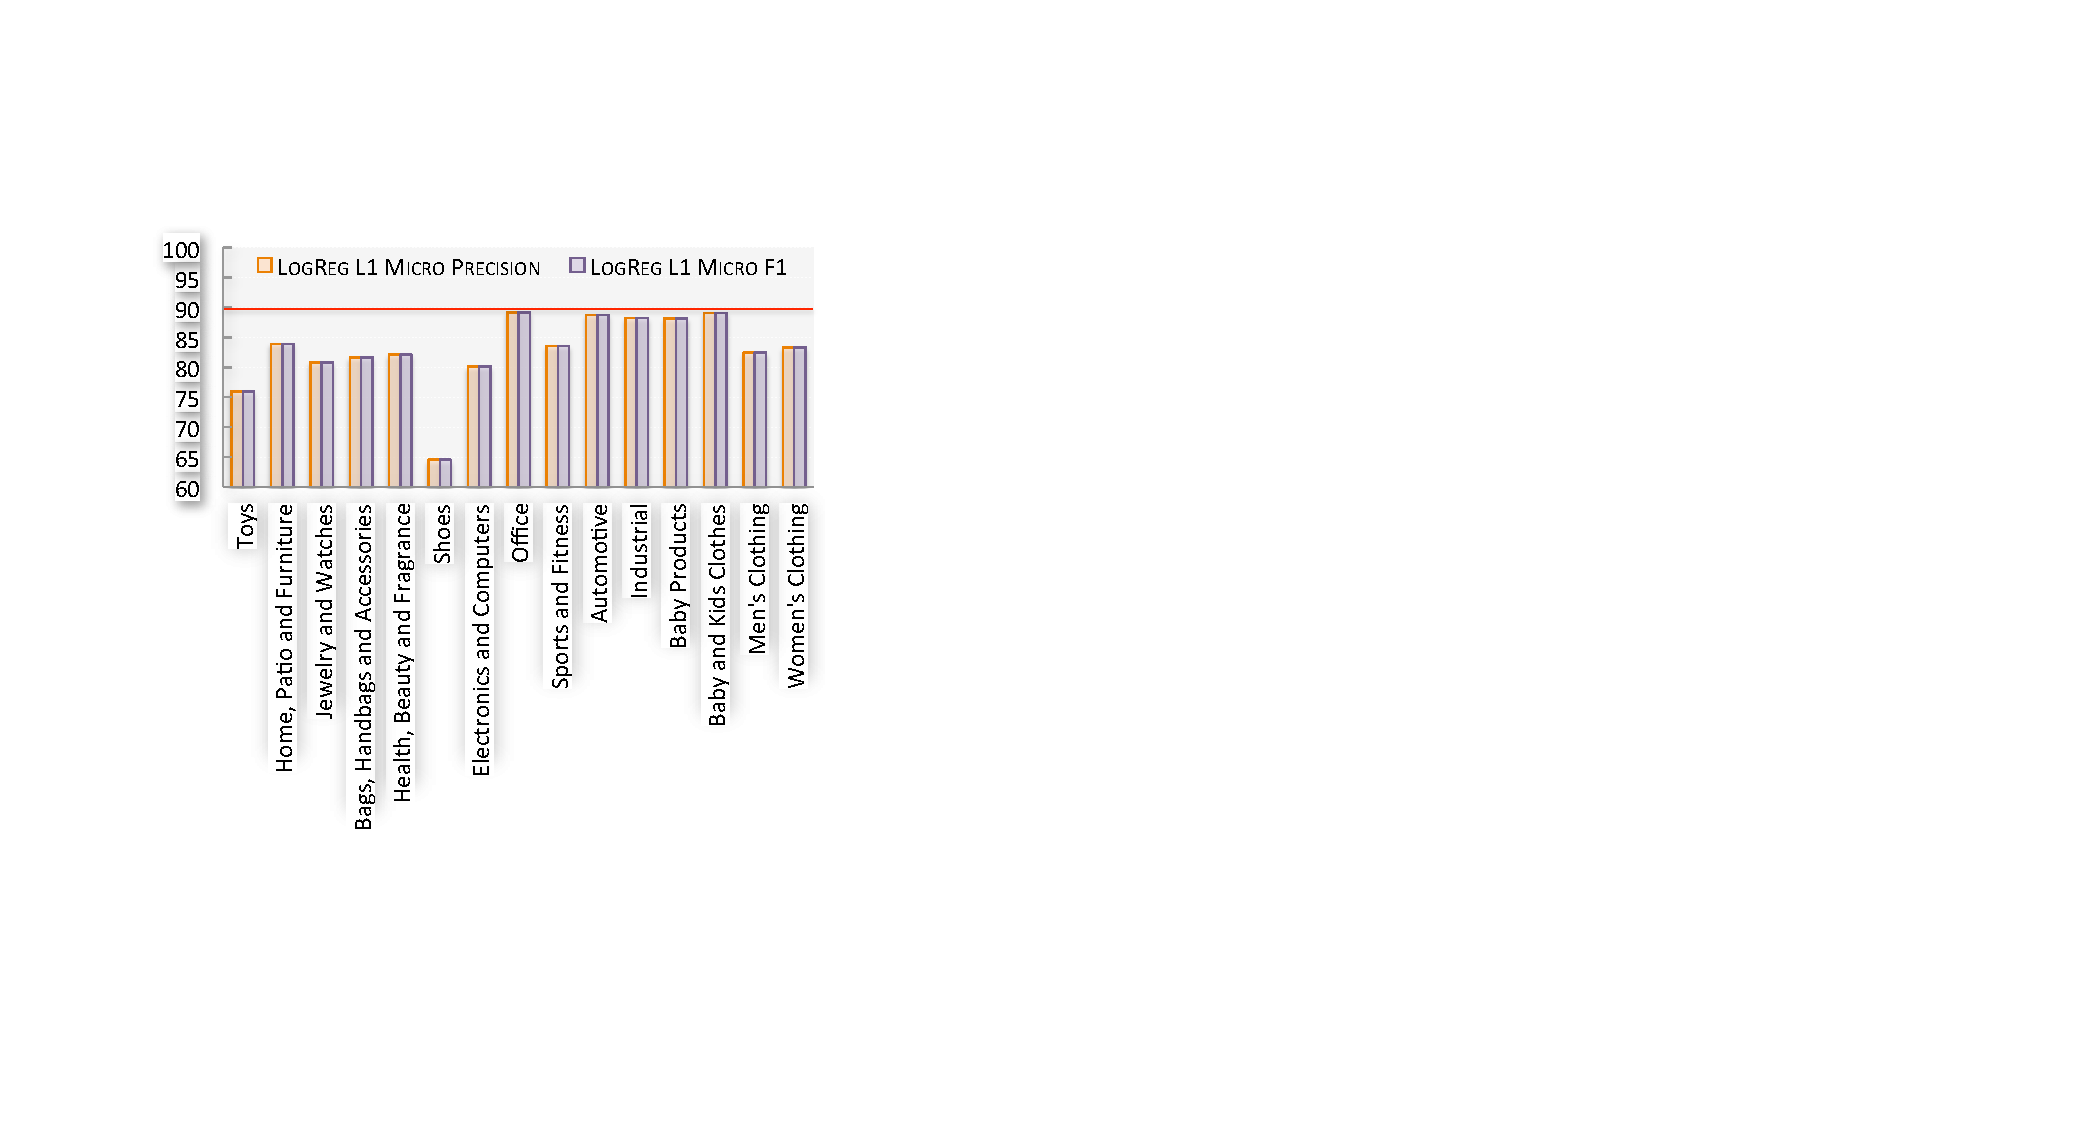
\includegraphics[width=0.45\textwidth]{images/BU2-Dec2015-LogRegL1}
	\vspace{-0.6cm}
	\caption{{\small Micro precision and micro F1 across 15 top level categories obtained using 10\% of the 40 million listings as test set for the dataset in the left }}
	\label{Figure_BU2-WUC-LogRegL1}
	\vspace{-0.4cm}
\end{wrapfigure}
However, this scheme may not be a good idea for Gradient Boosted Tree (henceforth GBT) \cite{Friedman:GBT} classification when number of instances is sparse compared to branch fan-out factor at level one (see Section \ref{Sect:results}).

Our initial experiments using the noisy data in Fig. \ref{Figure_BU2-datset-earlier} using a one vs. one logistic regression model with L1 regularization \cite{Yu13:EBay,LibShortText} show promising results but they do not attain a business requirement of $90\% \pm \epsilon$  mean micro precision across the level one taxonomies. 
Logistic Regression (henceforth LogReg) with L1 achieves 83\% mean micro precision (F1 values differed only in the third decimal place) for 10\% test dataset consisting of 4 million listings.
The level zero classification is a much easier problem and most classifiers achieve 90\% micro precision and F1 for all of the datasets considered here with GBT and Convolutional Neural Networks (henceforth CNN) \cite{Kim14} performing the best with 92\%--94\% micro precision and micro F1s. 
Taxonomy classification of the listings in the branches of the ``Shoes'' taxonomy subtree has been very poor and this resulted in a novel way to identify the pattern of noise in whole of BU2's data using unsupervised modeling and minimal manual analysis (see Section \ref{Subsect:BU2-noise-analysis}).

\begin{figure}[h]
\centering
	\subfloat[{{\footnotesize BU1 branch stats}}]{\label{Fig:BU1-branches+KL}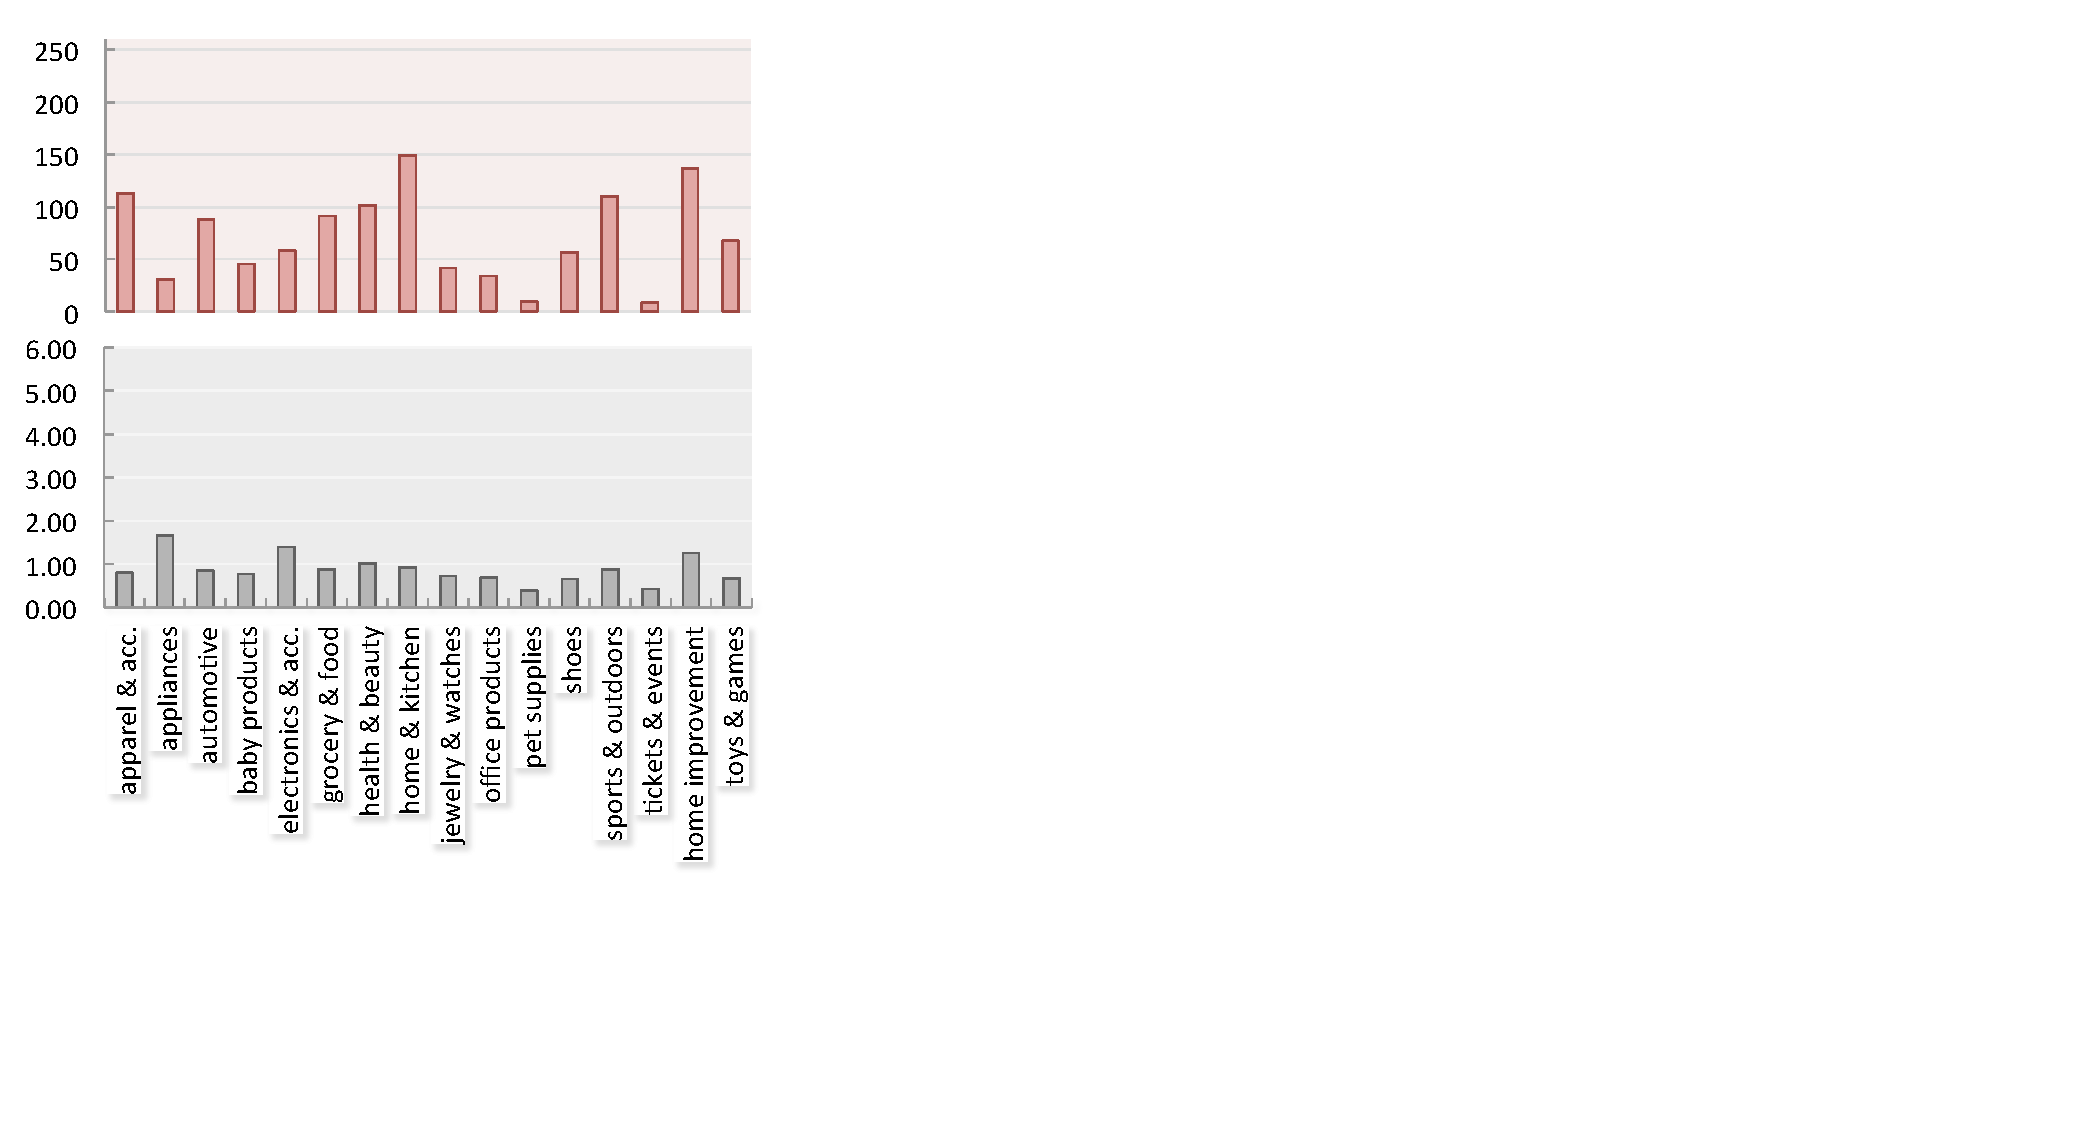
\includegraphics[width=0.3\textwidth]{images/BU1-branches+KL}} \hspace{0.01cm}
	\subfloat[{{\footnotesize AmazonJulian branch  stats}}]{\label{Fig:amazonj-branches+KL}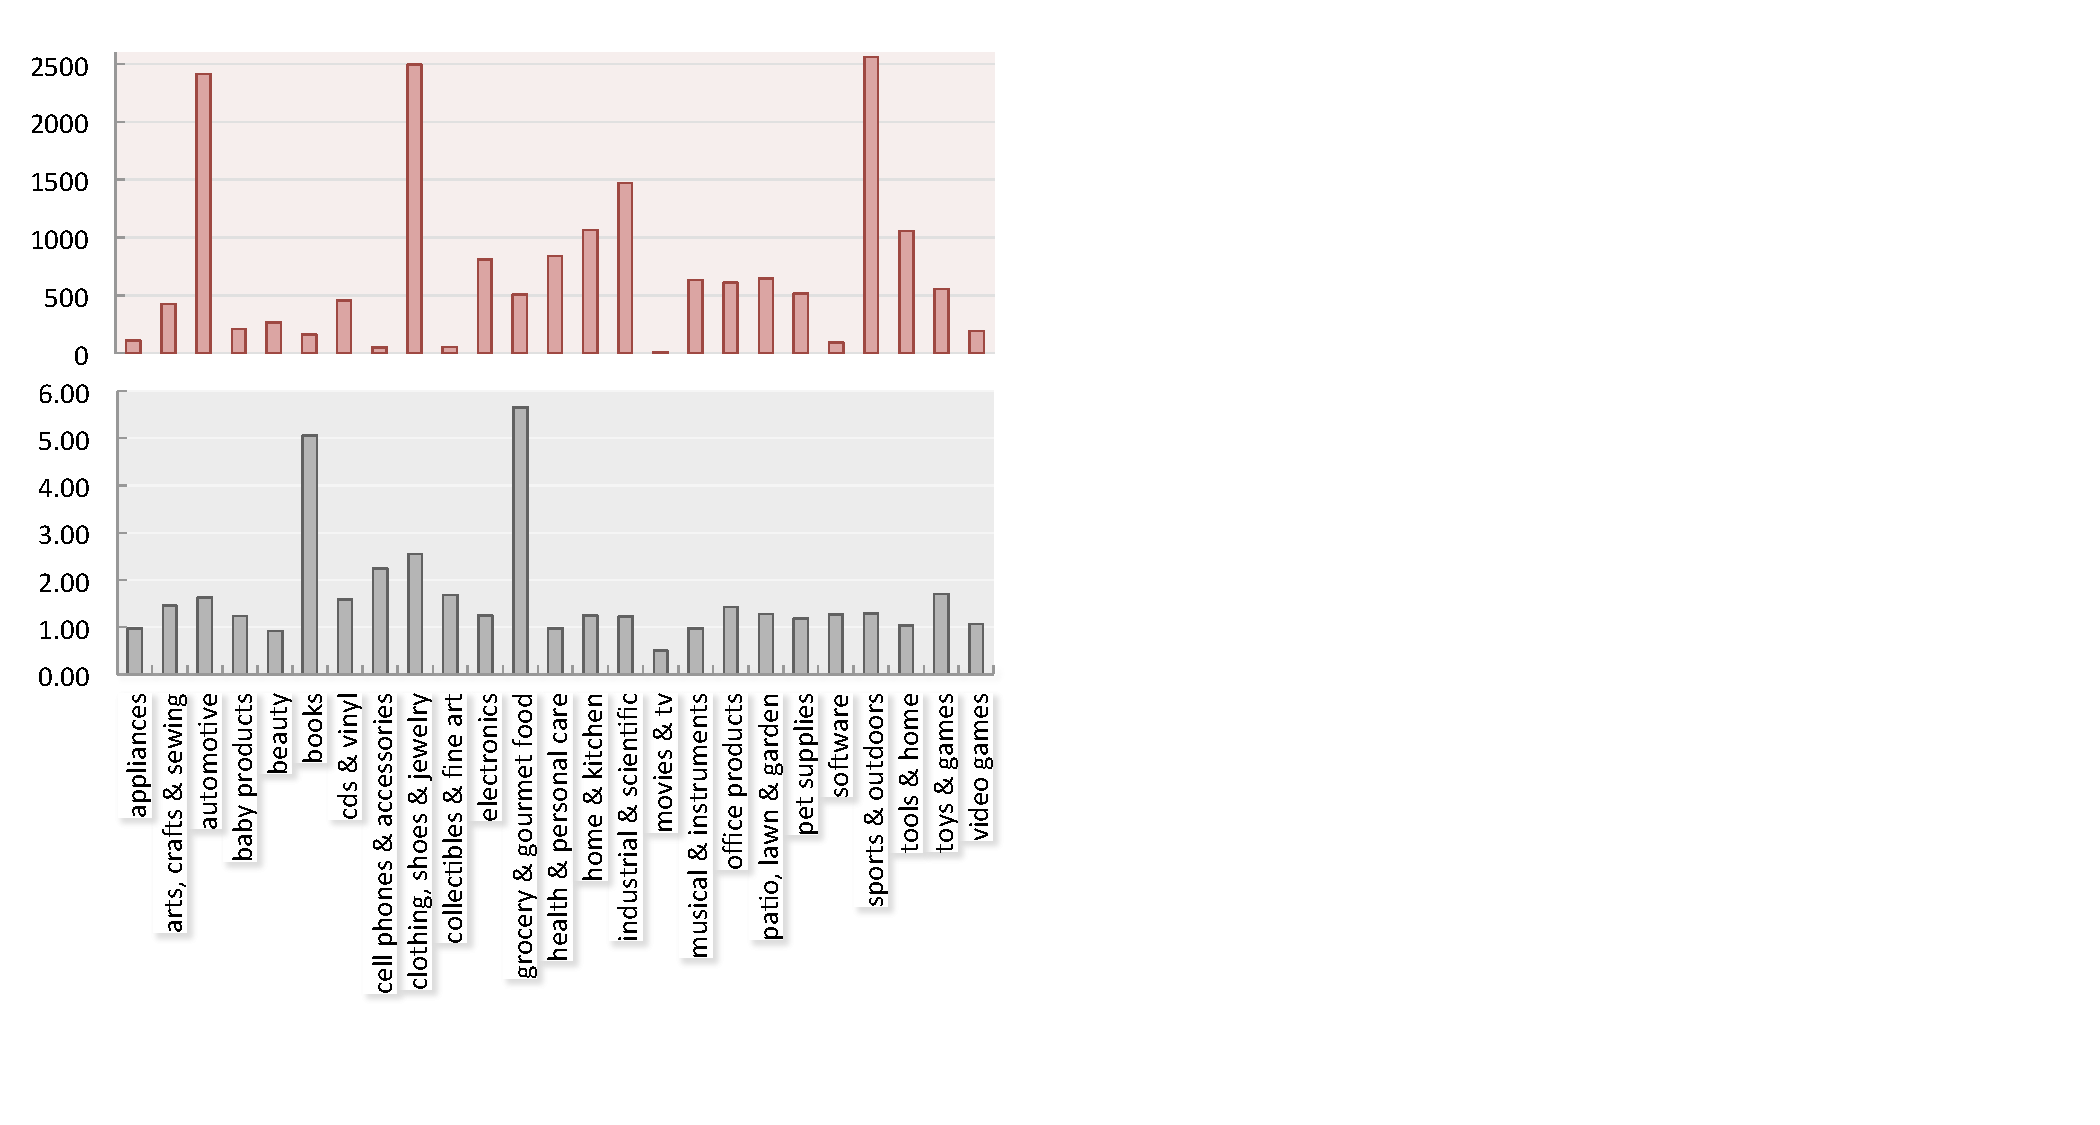
\includegraphics[width=0.37\textwidth]{images/AmazonJulian-branches+KL}} \hspace{0.01cm}
	\subfloat[{{\footnotesize BU2 branch stats}}]{\label{Fig:BU2-branches+KL}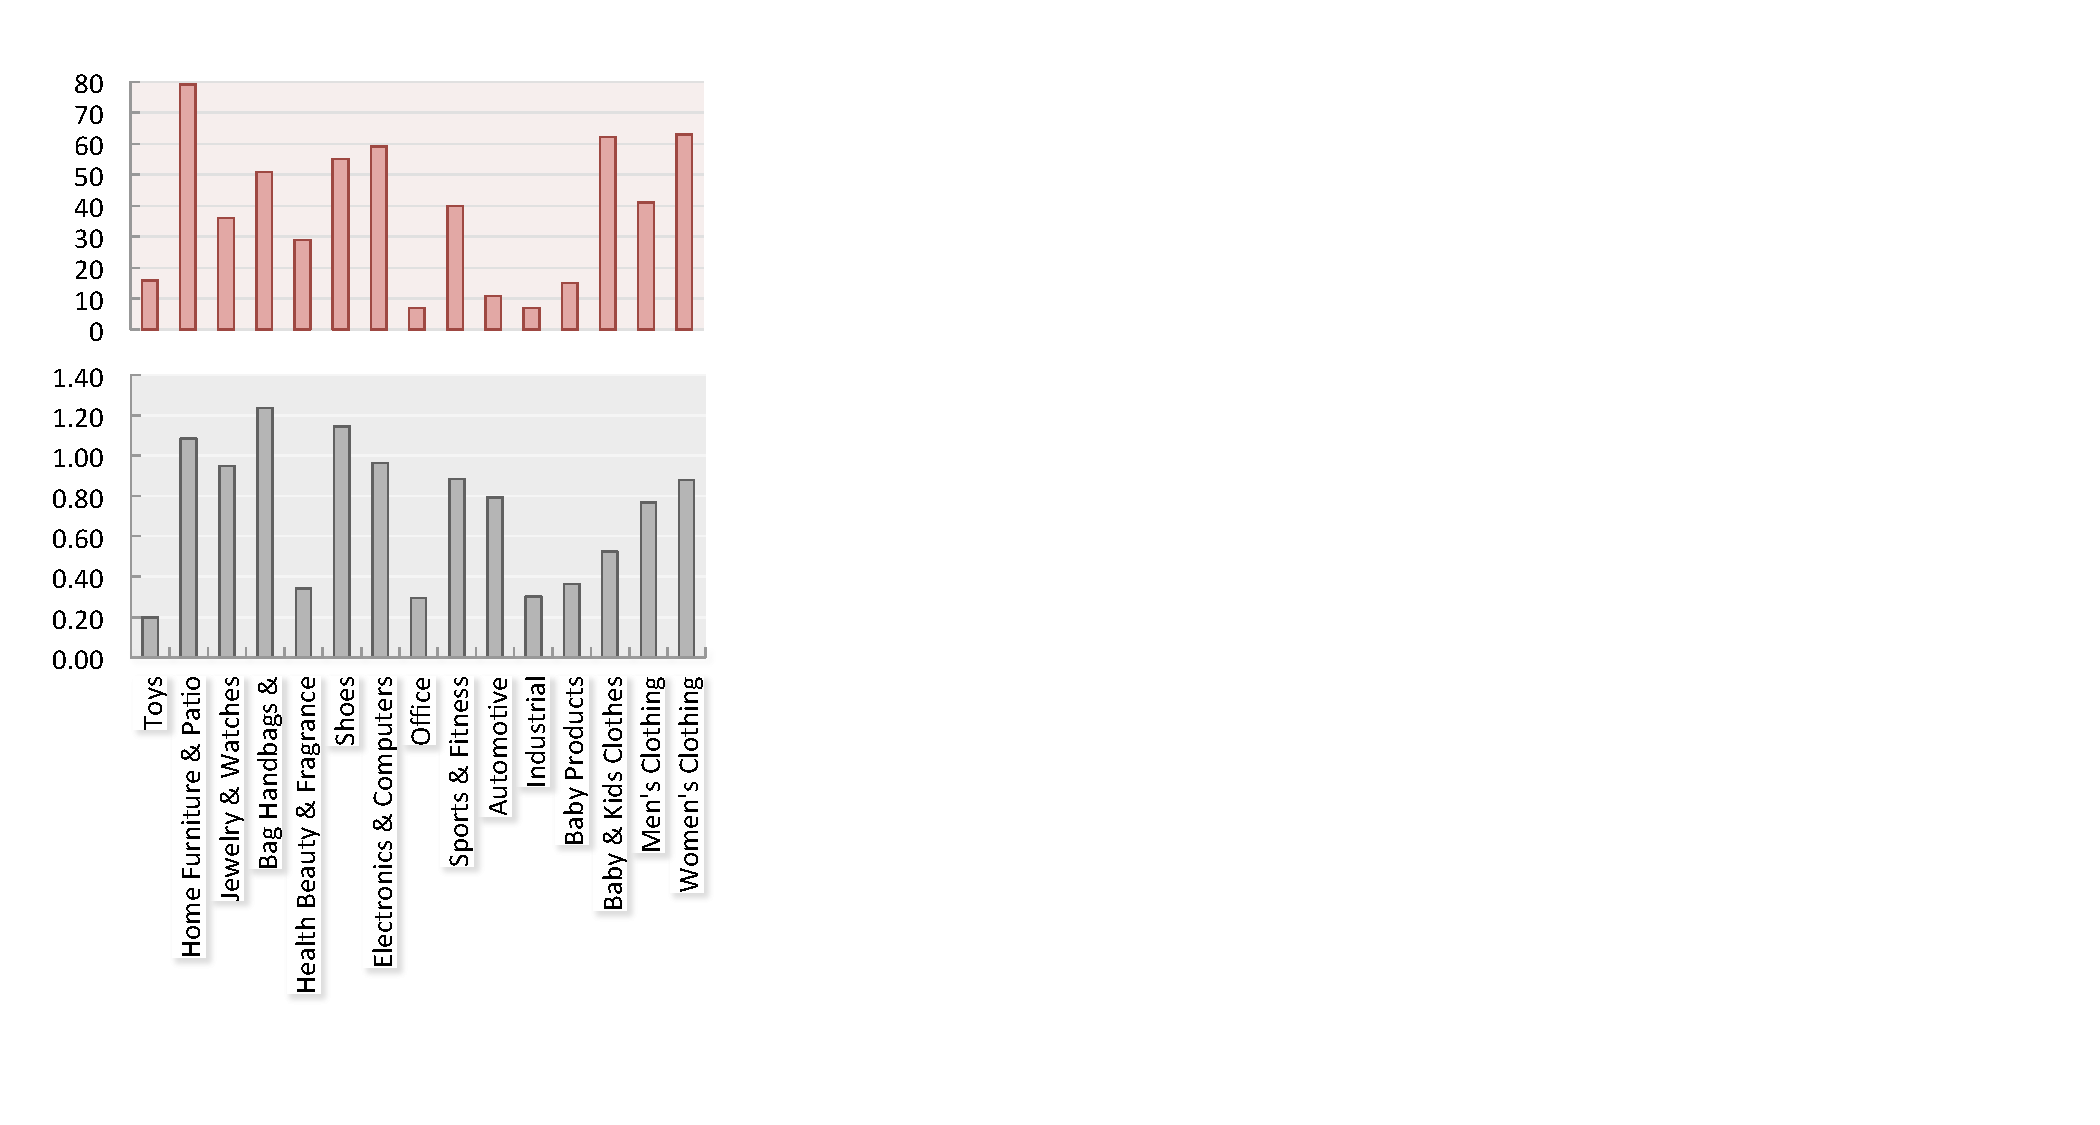
\includegraphics[width=0.26\textwidth]{images/BU2-branches+KL}} \hspace{0.01cm}
	\caption{{{\small Dataset Statistics. Best viewed under magnification.}} }
	\label{Fig:Dataset-statistics}
\end{figure}

Fig. \ref{Fig:Dataset-statistics} shows the number of branches and KL divergence from uniform of the three different datasets.
